\chapter{Negocio}
\section{Introducción}
Las descripciones arquitectónicas se centran en la estructura, lo que significa que las interrelaciones de las entidades dentro de una organización desempeñan un papel importante. Para hacerlo explícito, se ha introducido el elemento de la colaboración empresarial.\\

Se introduce el elemento de la interfaz empresarial para modelar explícitamente los lugares o canales (lógicos o físicos) en los que se puede acceder a los servicios que una función ofrece al entorno. El mismo servicio puede ofrecerse en varias interfaces diferentes; por ejemplo, por correo, por teléfono o a través de Internet. A diferencia de la modelización de aplicaciones, en los enfoques actuales de modelización de la capa empresarial no es frecuente reconocer el elemento de interfaz empresarial.
En la Capa de Negocio se definen tres tipos de elementos de estructura activa interna: actor comercial, papel comercial y colaboración comercial.\\

El aspecto de la estructura pasiva de la Capa de Negocios contiene los elementos de estructura pasiva (objetos de negocios) que son manipulados por el comportamiento, como los procesos o funciones de negocios. Las entidades pasivas representan los conceptos importantes en los que la empresa piensa en un dominio.
En la Capa de Negocios, hay dos tipos principales de elementos de estructura pasiva: objeto de negocio y representación. Además, un contrato, utilizado en el contexto de un producto, es una especialización de un objeto de negocio.

\newpage
\section{Metamodelo}

\begin{figure}[h!]
	\centering
	\begin{minipage}{1\textwidth} % choose width suitably
	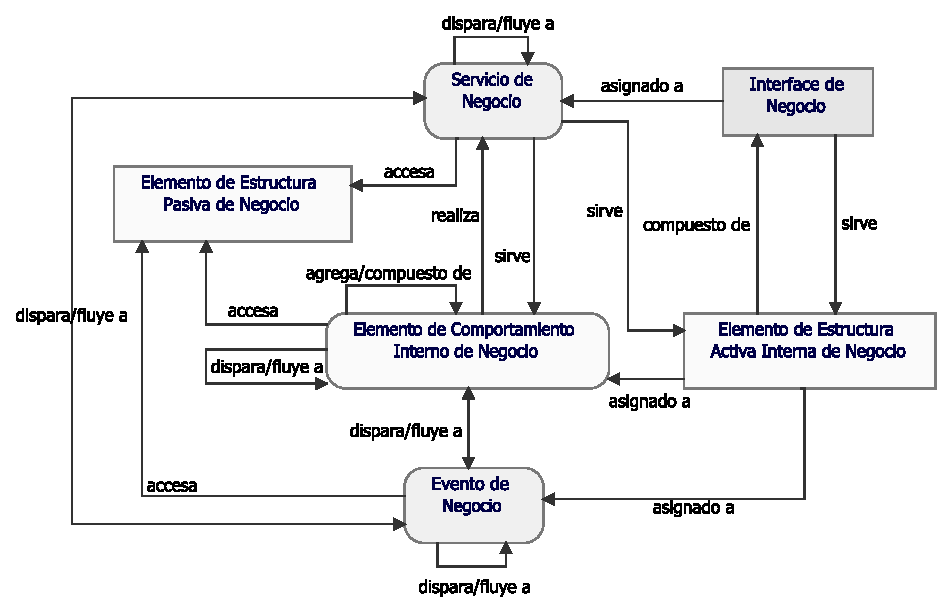
\includegraphics[width=0.9\linewidth]{imgs/meta/Negocio}
	\caption{Metamodelo Negocio}
	\label{fig:business}
	{\footnotesize Nota: Esta figura no muestra todas las relaciones permitidas; cada elemento del lenguaje puede tener relaciones de composición, agregación y especialización con elementos del mismo tipo; además, hay relaciones indirectas que pueden derivarse.\par}
	\end{minipage}
\end{figure}

La figura \ref{fig:business} ofrece una visión general de los elementos de la capa de negocios y sus relaciones. El elemento de estructura activa interna de la empresa, el elemento de comportamiento interno de la empresa y el elemento de estructura pasiva de la empresa son elementos abstractos; sólo sus especializaciones (como se definen en las siguientes secciones) se instancian en los modelos.

La Capa de Negocios se utiliza típicamente (a menudo en conjunto con los elementos de estrategia descritos en el Capítulo 5) para modelar la arquitectura de negocios de una empresa, definida por el marco del TOGAF como una descripción de la estructura e interacción entre la estrategia de negocios, la organización, las funciones, los procesos de negocios y las necesidades de información.

\newpage
\chapter{Empresa}
\section{Introducción}
En la evolución de la humanidad y las sociedades, la educación ha sido parte fundamental para lograr todo lo que el hombre ha conseguido. La educación ha sido el pilar fundamental sobre el cual se ha construido todos los grandes avances del hombre, toda la tecnología, descubrimientos e infinidad de saberes humanos han sido gracias a la educación, en principio transmitiendo los conocimientos de generación en generación por medio de simples relatos sin ningún tipo de organización y poco a poco este proceso de dar a otros conocimiento ha evolucionado al punto de tener una gran y compleja estructura, bien definida, que busca dar conocimientos por medio de la educación a la sociedad, como se puede evidenciar los colegios, institutos, universidades, etc. De igual manera, se necesita un organismo general que rija la forma de dar educación y que contenidos impartir, porque de lo contrario cada centro educativo enseñaría lo que a su entender le parezca mejor y la sociedad podría recibir diferentes enseñanzas que podrían ser contradictorias. En Colombia, este organismo que rige la educación es el Ministerio de Educación Nacional el cual, a través del tiempo y con el auge de la tecnología ha innovado y se ha adaptado poco a poco a los grandes beneficios que esta conlleva y por tal motivo una estrategia educativa y didáctica para instruir a las futuras generaciones es por medio de un juego, llevando al alumno a entender y comprender que lo compone y no simplemente jugar.

En consecuencia, el Ministerio de Educación Nacional será nuestro objeto de estudio con fines académicos para logar en una primera instancia, comprender su estructura organizacional como paso intermedio para brindar una solución optima a los requerimientos corporativos de la misma, mediante la implementación de los conceptos que iremos desarrollando a lo largo del presente espacio académico.


%\newpage
\section{Organización-Ministerio de Educación \\ Nacional (MEN)}
El Ministerio de Educación Nacional de Colombia es un ministerio de la República de Colombia encargado de formular la política de educación nacional y fomentar el desarrollo de una educación competitiva y de calidad que genere oportunidades de progreso y prosperidad y contribuya a cerrar las brechas de inequidad. Lo anterior, como propósito fundamental sin embargo, a lo largo del tiempo se ha ampliado su visión en busca de transversalidad con diversos campos como la tecnología o el agropecuario con el fin de mejorar cada vez más y más la educación en todos sus aspectos.
Su inicio fue mediante la Ley 10 de 1880 la cual creó la Secretaría de Instrucción Pública, que reemplazó a la Secretaría del Exterior (Ministerio de Gobierno) que antes de 1880 atendía los asuntos educativos.
Mediante la Ley 7 del 25 de agosto de 1886 se creó el Ministerio de Instrucción Pública, durante el gobierno del presidente José María Campo Serrano.
En junio de 1923, cambia el nombre de Ministerio de Instrucción Pública por el de Ministerio de Instrucción y Salubridad Públicas y, desde el 1º de enero de 1928 se le identifica con el nombre de Ministerio de Educación Nacional, según lo dispuso la Ley 56 de 1927 (10 de noviembre), siendo presidente de la República Miguel Abadía Méndez y ministro de Instrucción y Salubridad Públicas José Vicente Huertas. En la actualidad la Ministra de Educación Nacional es María Victoria Angulo desde 2018.

\section{Mision}
Liderar la formulación, implementación y evaluación de políticas públicas educativas, para cerrar las brechas que existen en la garantía del derecho a la educación, y en la prestación de un servicio educativo con calidad, esto en el marco de la atención integral que reconoce e integra la diferencia, los territorios y sus contextos, para permitir trayectorias educativas completas que impulsan el desarrollo integral de los individuos y la sociedad.

\section{Vision}
En 2022, a partir del gran pacto por una educación con enfoque integral desde la primera infancia y a lo largo de la vida, el Ministerio de Educación Nacional habrá liderado con responsabilidad social y financiera, transformaciones estructurales en el sistema educativo de Colombia dirigidas al mejoramiento progresivo de su capacidad para generar condiciones y oportunidades que favorezcan el desarrollo pleno de las personas y sus comunidades, soportado en el fortalecimiento de las capacidades sectoriales y territoriales requeridas para garantizar el cierre de brechas de acceso, permanencia y calidad en el entorno urbano y, especialmente en el rural.


\newpage
\section{Objetivos}

\subsection{General}
El Plan Nacional Decenal de Educación 2016-2026, PNDE 2016-2026 traza la ruta de Colombia en Educación en los próximos 10 años, hacia “un sistema educativo de calidad que promueva el desarrollo económico y social del país, y la construcción de una sociedad cuyos cimientos sean la justicia, el respeto y el reconocimiento de las diferencias”. Este documento surge de un proceso de construcción colectiva, con una amplia participación
municipal, departamental, regional y nacional, de los colombianos de todas las ciudades y etnias.

\subsection{Específicos}
Tomando como referencia el objetivo general, se definieron 10 lineamientos estratégicos que permitirán resolver los desafíos planteados a 2026, los cuales se
mencionan a continuación:

\begin{enumerate}
	\item Regular y precisar el alcance del derecho a la educación.
	\item Construcción de un sistema educativo articulado, participativo,
	descentralizado y con mecanismos eficaces de concertación.
	Plan Estratégico Institucional 2019-2022
	\item Establecimiento de lineamientos curriculares generales, pertinentes y flexibles.
	\item Construcción de una política pública para la formación de educadores.
	\item  Impulsar una educación que transforme el paradigma que ha dominado hasta el momento.
	\item Impulsar el uso pertinente, pedagógico y generalizado de las nuevas diversas tecnologías para apoyar la enseñanza, la construcción de conocimiento, el aprendizaje, la investigación y la innovación, fortaleciendo el desarrollo para la vida.
	\item Construir una red sociedad en paz sobre una base de equidad, inclusión, respeto a la ética y equidad de género.
	\item Dar prioridad al desarrollo de la población rural a partir de la educación.
	\item La importancia otorgada por el estado a la educación se medirá por
	la participación del gasto educativo en el PIB y en el gasto del Gobierno, en todos sus niveles administrativos.
	\item Fomentar la investigación que lleve a la generación de conocimiento en todos los niveles de la educación.
\end{enumerate}


%\newpage
\section{Organigrama}

\begin{figure}[h!]
	\centering
	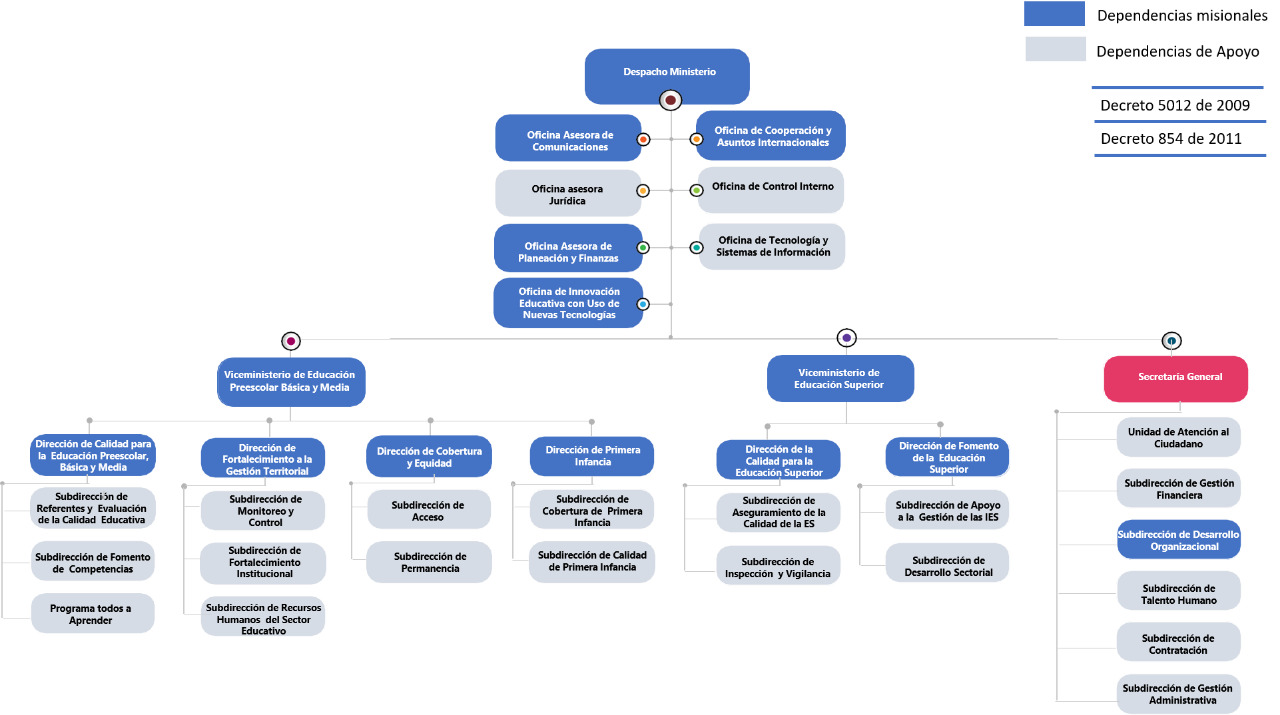
\includegraphics[width=1.1\linewidth]{imgs/organigrama.jpeg}
	\caption{Organigrama MEN}
\end{figure}


\section{Procesos}

\textbf{Procesos Estratégicos:}
\begin{itemize}
	\item Establecer el direccionamiento estratégico sectorial e institucional mediante la formulación y seguimiento de los planes, programas y proyectos, la gestión de la información del sector educación y la asignación de recursos financieros para dar cumplimiento a los objetivos institucionales y sectoriales.
	\item Administrar y mejorar el Sistema Integrado de Gestión, mediante el cumplimiento de los requisitos de los modelos referenciales en concordancia con el contexto estratégico de la entidad y una estructura organizacional que responda a las necesidades de modernización para posicionar el Ministerio de Educación como una entidad ejemplar en materia de gestión y desempeño.
	\item Realizar la difusión e intercambio oportuno, transparente y eficaz de mensajes e información del MEN con los diferentes grupos de interés, mediante la formulación, diseño y ejecución de planes y estrategias de comunicación, la asesoría en comunicación para la movilización, el relacionamiento y las acciones de divulgación y de sensibilización, CON EL FIN de promover la transparencia de la gestión institucional y el posicionamiento del Ministerio.
	\item Establecer alianzas estratégicas internacionales, nacionales, públicas y/o privadas, mediante la búsqueda de aliados, para la gestión de recursos técnicos, políticos, financieros e institucionales que contribuyan al logro de los objetivos misionales del MEN.
	\item Gestionar los recursos de tecnología de la información y las comunicaciones como un factor estratégico generador de valor para la Entidad y el sector educación, mediante la adopción del marco legal para el estado colombiano en materia de TIC, con el fin que las estrategias y proyectos adoptados faciliten a los usuarios el acceso, el uso eficiente y el aprovechamiento de las TIC.
	\item Capitalizar el conocimiento clave del Ministerio mediante su identificación, creación, disposición y socialización, para contribuir al aprendizaje organizacional y la innovación en la prestación de servicios y la ejecución de los procesos.
\end{itemize}

\textbf{Procesos Misionales:}

\begin{itemize}
	\item Diseñar la política pública de educación y sus instrumentos, mediante la identificación de necesidades del país en esta materia y la definición de líneas estratégicas de desarrollo que contribuyan a hacer de Colombia la mejor educada.
	\item Garantizar el logro de los objetivos y metas propuestos en materia de educación, mediante el desarrollo de actividades relacionadas con la ejecución de programas y proyectos, la prestación del servicio de asistencia técnica, el aseguramiento de la calidad y monitoreo, para lograr una educación de calidad eficiente y pertinente.
	\item Definir los lineamientos a tener en cuenta dentro del Ministerio de Educación Nacional cuando se requiera evaluar una política, programa, plan, proyecto, estrategia, acción o un instrumento de política de educación.
	\item Brindar atención a las partes interesadas del MEN, mediante respuestas de calidad, pertinentes y oportunas de las PQRSD, trámites y servicios, a través de canales de comunicación institucionales, con el fin de favorecer la satisfacción de las partes interesadas.
\end{itemize}

\textbf{Procesos de evaluación:}
\begin{itemize}
	\item Evaluar objetiva e independientemente la eficacia, eficiencia y efectividad del sistema integrado de gestión, mediante el desarrollo y seguimiento de las actividades previstas, para fortalecer el autocontrol, la autorregulación y la autogestión del MEN, de conformidad con la normatividad vigente.
	\item Ejercer el control interno disciplinario mediante el cumplimiento de los requisitos normativos.
\end{itemize}

\section{Servicios}

\begin{itemize}
	\item \textbf{Asistencia técnica:} Actividades que se ejecutan para transferir el conocimiento, fortalecer capacidades y desarrollar competencias que propicien prácticas de buen gobierno, faciliten la implementación de la política y mejoren la prestación del servicio educativo, en condiciones de eficiencia, calidad y pertinencia; mediante mecanismos o estrategias de capacitación, asesoría, acompañamiento presencial o virtual, entre otros.
	\item \textbf{Evidencias documentales de asistencia técnica:} Actas de visita o de reunión, listados de asistencia, correos electrónicos, comunicaciones de respuesta a inquietudes, que dan cuenta de que los temas cubrieron las necesidades identificadas y los compromisos objeto de seguimiento por parte del Ministerio de Educación Nacional.
	\item \textbf{Proyectos Ejecutados:} Proyectos Ejecutados en el Ministerio de Educación Nacional, donde se tienen en cuenta los resultados de estos y el impacto en la población objetivo.
	\item \textbf{Trámite de aseguramiento de la calidad:} Hace referencia a los diferentes trámites que se realizan en el Ministerio de Educación Nacional los cuales son: 1 Autorización de creación de seccionales de instituciones de educación superior, 2 Certificación de existencia y representación legal de instituciones de educación superior, 3 Certificación de programa académico de instituciones de educación superior, 4 Redefinición para el Ofrecimiento de Programas por Ciclos Propedéuticos, 5 Reconocimiento de Personería Jurídica de las instituciones de educación superior privadas, 6 Reconocimiento como Universidad de una institución universitaria o escuela tecnológica privada u oficial, 7 Ratificación de reformas estatutarias para institución de educación superior privada, 8 Registro e inscripción de rectores y representantes legales de institución de educación superior IES, 9 Registro calificado, 10 Convalidación de estudios de preescolar, básica y media realizados en el exterior, 11 Certificado de idoneidad del título de postgrado para ascender al grado 14 del escalafón, 12 Convalidación de títulos de estudios de pregrado otorgados en el exterior, 13 Acreditación de alta calidad de Programa Académico de Institución de Educación Superior, 14 Aprobación del estudio de factibilidad socioeconómica en la creación de instituciones de educación superior estatales u oficiales, 15 Legalización de documentos de educación superior para adelantar estudios o trabajar en el exterior, 16 Convalidación de títulos de estudios de posgrado obtenidos en el exterior, 17 Cambio de carácter académico. 18. Reconocimiento de intérpretes oficiales de lengua de señas colombiana - español. 19. Convocatoria beca ser.
	\item \textbf{Apertura de investigación:} Acto administrativo que pone de manifiesto la existencia o comisión de los actos constitutivos de falta administrativa señalados en esta ley.
	\item \textbf{Respuesta a Peticiones, Quejas, Reclamos, Sugerencias - PQRS:} Comunicación realizada al peticionario dando respuesta a la Petición, Queja, Reclamo, Sugerencia - PQRS interpuesta.
	\item \textbf{Atención a la ciudadanía:} Atención prestada por los canales de atención de la Unidad de Atención al Ciudadano del Ministerio de Educación Nacional (presencial, telefónica, chat).
\end{itemize}

\section{Productos}
\begin{itemize}
	\item \textbf{Documento de política pública en educación:} Documentos de política pública en educación: Leyes, Decretos, Conpes, Actos Administrativos, documentos de directrices o lineamientos de política pública en Educación.
	\item \textbf{Documento mediante el cual se establece un instrumento de política pública en educación:} Documentos mediante los cuales se establecen instrumentos de política pública en educación: Actos administrativos, guías, manuales, documentos de directrices, lineamientos, metodologías sobre instrumentos de política pública en Educación. Los tipos de instrumentos de política se encuentran definidos en el Proceso Diseño de Política e Instrumentos de Política del Ministerio de Educación Nacional.
	\item \textbf{Documento de evaluación de política pública o de instrumentos de política pública en educación:} Documento de evaluación de política pública o de instrumentos de política pública en educación. 
	\item \textbf{Video juego para aprender inglés desde casa:} Aplicación digital de nombre \#BThe1Challenge, con la finalidad de ayudar a las personas en el proceso de aprender inglés y de una forma lúdica e interactiva, es un videojuego educativo descargable en tabletas y celulares Android, desarrollado por el Programa Nacional de Bilingüismo de la cartera, en compañía del British Council, con el fin de que "los estudiantes tengan más herramientas de aprendizaje durante el desarrollo de sus actividades académicas no presenciales". El juego está diseñado 100\% en inglés, dirigido a estudiantes de grados 6. ° a 11. ° de instituciones educativas oficiales del país. Estos podrán acceder a la aplicación descargándola a través de la tienda Google Play Store. La idea es que, ya inscritos en el juego, recuperen los objetos ocultos por una fórmula creada por la científica y filántropa Margaret Winter, quien es el personaje creado para esta historia.
\end{itemize}

\section{Requerimientos}
contenido...

\section{Valores Corporativos}
Los Valores del Ministerio de Educación Nacional son las formas de ser y de actuar de los servidores públicos y colaboradores, los cuales se consideran altamente deseables como atributos o cualidades suyas, por cuanto posibilitan la aplicación de los principios éticos y el cabal cumplimiento de los mandatos constitucionales y legales en su desempeño laboral. Los valores del Ministerio son: 


\textbf{Compromiso:} \\
Consciencia de la importancia del rol como servidor público y disposición permanente para comprender y resolver las necesidades de las personas con las que se comparten las labores cotidianas, buscando siempre mejorar su bienestar. \\

\textbf{Lo que hago: }
\begin{itemize}
	\item Atiendo con amabilidad, igualdad y equidad a todas las personas en cualquier situación a través de mis palabras, gestos y actitudes, sin importar su condición social, económica, religiosa, étnica o de cualquier otro orden. Soy amable todos los días, esa es la clave, siempre.
	\item Siempre estoy dispuesto a ponerme en los zapatos de las personas. Entender su contexto, necesidades y requerimientos es el fundamento de mi servicio y labor. 
	\item Escucho, atiendo y oriento a quien necesite cualquier información o guía en algún asunto público. 
	\item Estoy atento siempre que interactúo con otras personas, sin distracciones de ningún tipo. 
\end{itemize}

\textbf{Lo no que hago: }
\begin{itemize}
	\item Trabajar con una actitud negativa. No se vale afectar mi trabajo por no ponerle ganas a las cosas. 
	\item Pensar que mi trabajo como servidor es un “favor” que le hago a la ciudadanía. Es un compromiso y un orgullo. 
	\item Asumir que mi trabajo como servidor es irrelevante para la sociedad.
	\item Ignorar a un ciudadano y sus inquietudes. 
\end{itemize}

El elemento característico de la cultura del MEN que refleja el compromiso es la “Conexión”. \\

\textbf{Honestidad: } \\
Actuar siempre con fundamento en la verdad, cumpliendo los deberes con transparencia y rectitud, favoreciendo el interés general. \\

%\newpage
\textbf{Lo que hago: }
\begin{itemize}
	\item Siempre digo la verdad, incluso cuando cometo errores, porque es humano cometerlos, pero no es correcto esconderlos. 
	\item Cuando tengo dudas respecto a la aplicación de mis deberes busco orientación en las instancias pertinentes al interior de mi entidad. Se vale no saberlo todo, y también se vale pedir ayuda. 
	\item Facilito el acceso a la información pública completa, veraz, oportuna y comprensible a través de los medios destinados para ello.  
	\item Denuncio las faltas, delitos o violación de derechos de los que tengo conocimiento en el ejercicio de mi cargo, siempre. 
	\item Apoyo y promuevo los espacios de participación para que los ciudadanos hagan parte de la toma de decisiones que los afecten relacionadas con mi cargo o labor.  
\end{itemize}

\textbf{Lo no que hago: }
\begin{itemize}
	\item Dar trato preferencial a personas cercanas para favorecerlos en un proceso, porque debe prevalecer la igualdad de condiciones. 
	\item Aceptar incentivos, favores, y cualquier otro tipo de beneficio que me ofrezcan personas o grupos que estén interesados en un proceso de toma de decisiones. 
	\item Usar recursos públicos para fines personales relacionados con mi familia, mis estudios y mis pasatiempos (esto incluye el tiempo de mi jornada laboral, los elementos y bienes asignados para cumplir con mi labor, entre otros). 
	\item Ser descuidado con la información a mi cargo, o con su gestión. 
\end{itemize}

El elemento característico de la cultura del MEN que refleja la honestidad y el respeto es la “Comunicación”. \\

\textbf{Diligencia: } \\
Cumplimiento de los deberes, funciones y responsabilidades asignadas de la mejor manera posible, con atención, prontitud y eficiencia, para así optimizar el uso de los recursos del Estado. \\

%\newpage
\textbf{Lo que hago: }
\begin{itemize}
	\item Uso responsablemente los recursos públicos para cumplir con mis obligaciones. Lo público es de todos y no se desperdicia. 
	\item Cumplo con los tiempos estipulados para el logro de cada obligación laboral. A fin de cuentas, el tiempo de todos es oro. 
	\item Aseguro la calidad en cada uno de los productos que entrego bajo los estándares del servicio público. No se valen cosas a medias. 
	\item Aseguro la calidad en cada uno de los productos que entrego bajo los estándares del servicio público. No se valen cosas a medias. 
\end{itemize}

\textbf{Lo no que hago: }
\begin{itemize}
	\item Malgastar el recurso público. 
	\item Postergar las decisiones y actividades que den solución a problemáticas ciudadanas o que hagan parte del funcionamiento de mi cargo. Hay cosas que sencillamente no se dejan para otro día. 
	\item Demostrar desinterés en mis actuaciones ante los ciudadanos y los demás servidores públicos. 
	\item Evadir mis funciones y responsabilidades. 
	\item Trasladar los problemas y responsabilidades a otras dependencias, siempre aporto a la solución.
\end{itemize}


\textbf{Justicia: } \\
Actuar con imparcialidad, garantizando los derechos de las personas, con equidad, igualdad y sin discriminación. 

\textbf{Lo que hago: }
\begin{itemize}
	\item Tomo decisiones informadas y objetivas basadas en evidencias y datos confiables. Es muy grave fallar en mis actuaciones por no tener las cosas claras. 
	\item Reconozco y protejo los derechos de cada persona de acuerdo con sus necesidades y condiciones. 
	\item Tomo decisiones estableciendo mecanismos de diálogo y concertación con todas las partes involucradas.  
\end{itemize}

\textbf{Lo no que hago: }
\begin{itemize}
	\item Promover y ejecutar políticas, programas o medidas que afectan la igualdad y la libertad de personas. 
	\item Favorecer el punto de vista de un grupo de interés sin tener en cuenta a todos los actores involucrados en una situación. 
	\item Permitir que odios, simpatías, antipatías, caprichos, presiones o intereses de orden personal o grupal interfieran en mi criterio, toma de decisión y gestión pública. 
	\item Dar un trato inequitativo a nuestros usuarios y prelaciones indebidas para favorecer alguna persona. 
\end{itemize}

El elemento característico de la cultura del MEN que refleja la diligencia y la justicia es el “Servicio”. \\

\textbf{Mística: } \\
Actuar con sentido y amor por lo que hacemos. Amor al trabajo, a la Entidad, a los compañeros y a los superiores, propendiendo por un ambiente integro. \\

\textbf{Lo que hago: }
\begin{itemize}
	\item Desarrollo mis actividades con pasión entusiasta.  
	\item Reflejo lo mejor de mí en cada labor.  
	\item Busco trascender en los demás y dar un valor agregado. 
	\item Tengo sentido de pertenencia. 
\end{itemize}

\textbf{Lo no que hago: }
\begin{itemize}
	\item Actuar de manera desinteresada por el logro de los objetivos. 
	\item Falta de escucha y de no conocer las personas, personalidades y desconocer el bien común.
\end{itemize}

\textbf{Confianza: } \\
Creer en los demás, confiar en nuestro trabajo y en nuestros grupos de interés. \\

%\newpage
\textbf{Lo que hago: }
\begin{itemize}
	\item Tengo la certeza de cómo lograremos el cumplimiento de las metas. 
	\item Genero un ambiente de trabajo basado en la apertura, escucha y comunicación.  
	\item Actúo confiado en pro de los objetivos del equipo y/o de la Entidad.  
\end{itemize}

\textbf{Lo no que hago: }
\begin{itemize}
	\item Generar incertidumbre faltando a la verdad y afectando la toma de decisiones. 
	\item Atentar contra los principios de credibilidad de los procesos a cargo. 
	\item Actuar con inseguridad, resistencia y temor a los cambios.
\end{itemize}

\section{Principios Corporativos}

\textbf{Principios de Integridad} \\
En el marco de la Integridad Pública, los servidores del Ministerio de Educación Nacional asumen los siguientes principios de Integridad: 

\begin{enumerate}
	\item El interés general prevalece sobre el interés particular. 
	\item Los bienes y recursos públicos están destinados exclusivamente para asuntos de interés general. 
	\item  La función primordial del servidor público es servir a la ciudadanía. 
	\item Quien administra recursos públicos rinde cuentas a la sociedad sobre su utilización y los resultados de su gestión.
	\item . Los ciudadanos tienen derecho a participar en las decisiones públicas que los afecten.
\end{enumerate}


\clearpage
\section{Punto de Vista de Cooperación de Actor}


\subsection{Modelo de Cooperación de Actor}
\begin{figure}[h!]
	\centering
	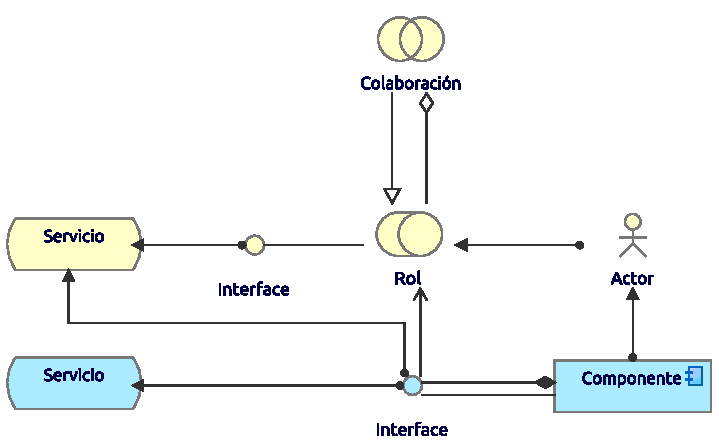
\includegraphics[width=.6\linewidth]{imgs/modelo/CoopActor.pdf}
	\caption{Modelo Cooperacion de Actor}
\end{figure}

El punto de vista de cooperación de actor establece las colaboraciones que existen internamente y externamente sobre un actor o rol de la organización con el fin de mostrar de qué manera interactuan e interfiere con el actor en cuestión. Por medio de interfaces  que comunican los entes del exterior y el interior de la organización con el actor o rol.

\newpage
\subsection{Caso  de Cooperación de Actor}
\begin{figure}[h!]
	\centering
	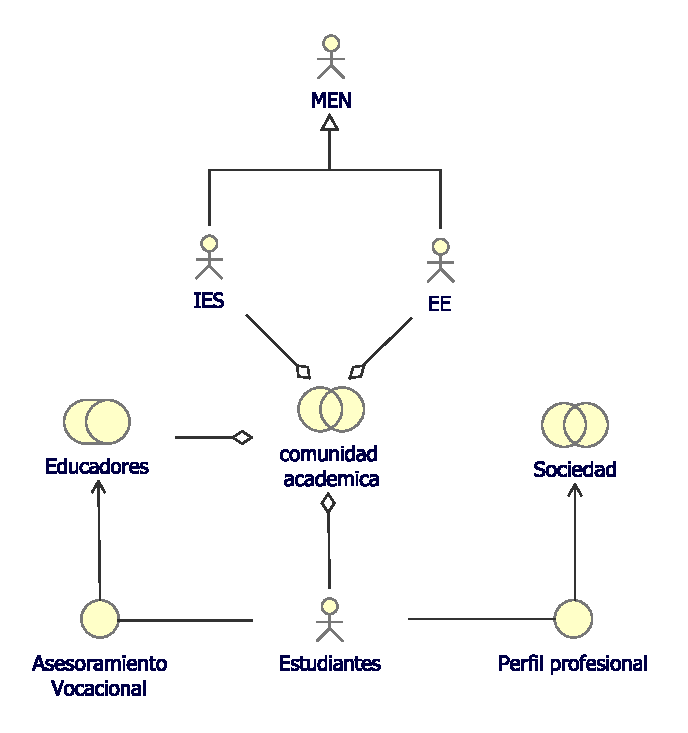
\includegraphics[width=.8\linewidth]{imgs/caso/negocio/coperacion_actor.pdf}
	\caption{Caso Cooperacion de Actor}
\end{figure}

Para nuestro objeto de estudio en relación al punto de vista de colaboración de actor tenemos como actor principal a los estudiantes aquellos que colaboran en la comunidad académica y hacen parte de las IES y EE que son regidas por el Ministerio de Educación. Por otro lado tenemos el rol de educador que hace parte de la comunidad y que puede ayudar a guiar en parte la vocación que construirá en un futuro el estudiante. Los estudiantes contribuirán en la sociedad gracias a su perfil que se ha formado durante sus años de estudio y que permitirán a las empresas apoderarse de estos individuos y así lograr mejores avances que colaboren en su entidad y por tanto a la sociedad misma.

\clearpage
\section{Punto de Vista de función de Negocio}

El punto de vista de la cooperación de los procesos comerciales se utiliza para mostrar las relaciones de uno o más procesos comerciales entre sí y/o con su entorno. Puede utilizarse tanto para crear un diseño de alto nivel de los procesos empresariales dentro de su contexto como para proporcionar a un director operacional responsable de uno o más de esos procesos una visión de sus dependencias. Los aspectos importantes de la cooperación en los procesos empresariales son:

\begin{itemize}
	\item Relaciones causales entre los principales procesos comerciales de la empresa
	\item Mapeo de los procesos comerciales en las funciones comerciales
	\item Realización de servicios por procesos comerciales
	\item Uso de datos compartidos
\end{itemize}

Cada una de ellas puede considerarse un "subpunto de vista" del punto de vista de la cooperación en los procesos comerciales.

\subsection{Modelo de función de Negocio}
\begin{figure}[h!]
	\centering
	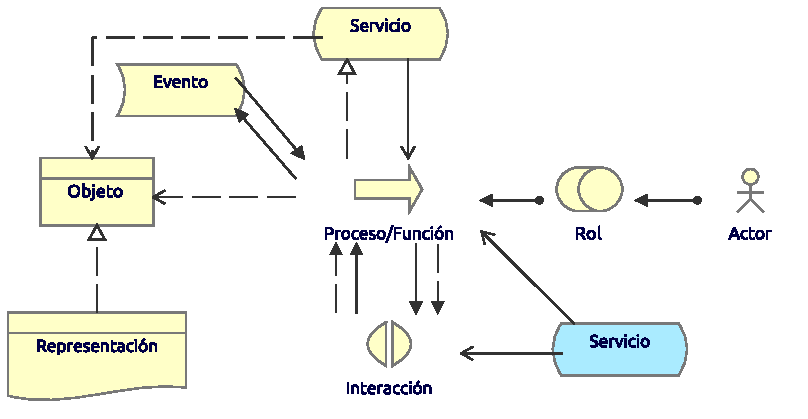
\includegraphics[width=.8\linewidth]{imgs/modelo/ProcesoNegocio}
	\caption{Modelo función de Negocio}
\end{figure}

Un proceso empresarial representa una secuencia de comportamientos empresariales que logra un resultado específico, como un conjunto definido de productos o servicios empresariales.
Un proceso de negocios describe el comportamiento interno realizado por un rol de negocios que se requiere para producir un conjunto de productos y servicios. Para un consumidor, los productos y servicios son relevantes y el comportamiento requerido es meramente una caja negra, de ahí la designación "interno".
Un proceso comercial complejo puede ser una agregación de otros procesos de grano más fino. A cada uno de ellos se le pueden asignar funciones más finas.
Existe una relación potencial de muchos a muchos entre los procesos de negocios y las funciones de negocios. En términos informales, los procesos describen algún tipo de "flujo" de actividades, mientras que las funciones agrupan las actividades según las aptitudes, los conocimientos, los recursos, etc. requeridos. Un proceso empresarial puede ser desencadenado por, o desencadenar, cualquier otro elemento de comportamiento empresarial (por ejemplo, un acto empresarial, un proceso empresarial, una función empresarial o una interacción empresarial). Un proceso empresarial puede acceder a objetos empresariales. Un proceso empresarial puede realizar uno o más servicios empresariales y pueden utilizar servicios comerciales (internos) o servicios de aplicación. Se puede asignar una función empresarial a un proceso empresarial para realizar este proceso manualmente. Un proceso empresarial automatizado puede realizarse mediante un proceso de aplicación. El nombre de un proceso empresarial debe indicar claramente una secuencia predefinida de acciones, y puede incluir la palabra "proceso". Ejemplos de ello son "adjudicar la reclamación", "incorporación de empleados", "proceso de aprobación" o "presentación de informes financieros". \\

Un objeto comercial representa un concepto utilizado dentro de un dominio comercial determinado. Un contrato representa una especificación formal o informal de un acuerdo entre un proveedor y un consumidor en el que se especifican los derechos y obligaciones asociados a un producto y se establecen parámetros funcionales y no funcionales para la interacción. Una representación representa una forma perceptible de la información que lleva un objeto comercial.

\clearpage
\subsection{Caso  de función de Negocio}
\begin{figure}[h!]
	\centering
	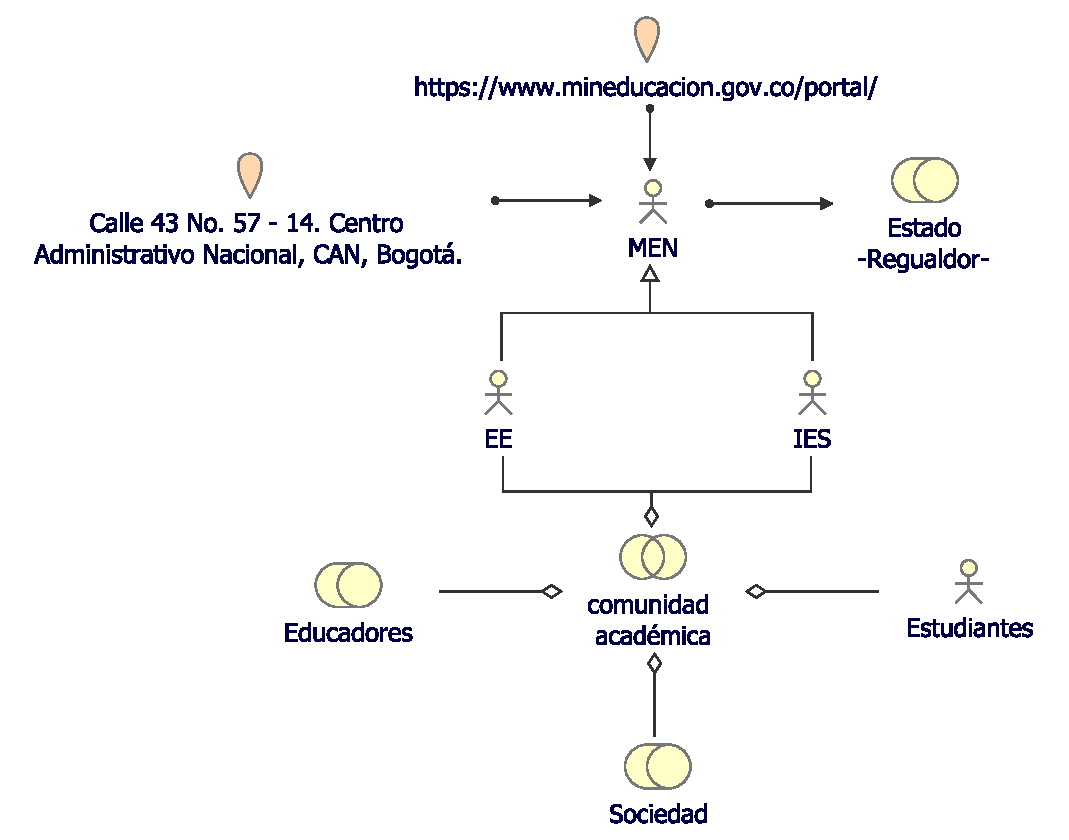
\includegraphics[width=.9\linewidth]{imgs/caso/negocio/organizacion}
	\caption{Caso función de Negocio}
\end{figure}
Un actor de negocios es una entidad de negocios que es capaz de realizar un comportamiento. Los actores pueden incluir entidades fuera de la organización real; por ejemplo, clientes y socios. Un actor comercial puede representar a esas entidades comerciales en diferentes niveles de detalle, y puede corresponder tanto a un actor como a una unidad organizativa en el marco del TOGAF. Ejemplos de actores comerciales son los seres humanos, los departamentos y las unidades comerciales. Una colaboración empresarial es un conjunto de dos o más elementos de la estructura activa interna de la empresa que trabajan juntos para llevar a cabo un comportamiento colectivo. Una interfaz de negocios es un punto de acceso en el que se pone a disposición del entorno un servicio comercial. Una interfaz comercial expone la funcionalidad de un servicio comercial a otros roles o actores comerciales. Se suele denominar canal (teléfono, Internet, oficina local, etc.). El mismo servicio comercial puede estar expuesto a través de diferentes interfaces.

\clearpage
\section{Punto de Vista de Proceso de Negocio}

El punto de vista del proceso de negocio, es en donde se definen los procesos organizacionales del proyecto, es decir, lo que se convertirá en el paradigma alrededor del cual la organización resuelve toda su misión, sus funciones, objetivos. En concreto es el Core en donde se determina la funcionalidad organizacional.
Este punto de vista contribuye al entendimiento real de lo que se requiere con el proyecto, es decir, su objetivo organizaciones, todo desde un punto de vista administrativo, dando una visión más amplia y completa a lo que se refiere con la finalidad del proyecto.

\subsection{Modelo de Proceso de Negocio}
\begin{figure}[h!]
	\centering
	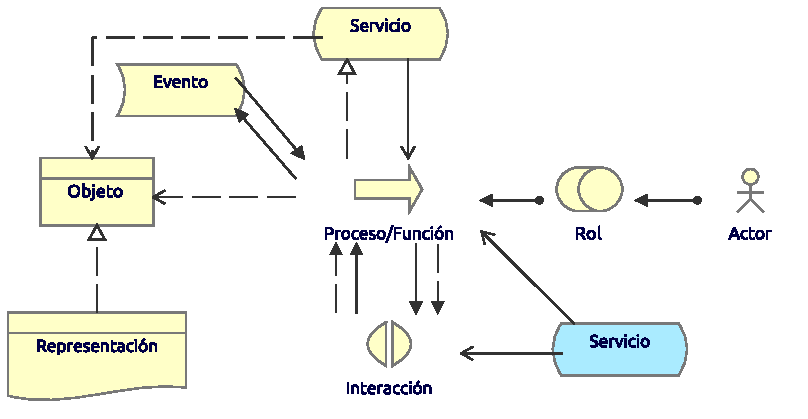
\includegraphics[width=.8\linewidth]{imgs/modelo/ProcesoNegocio}
	\caption{Modelo Proceso de Negocio}
\end{figure}

El modelo para el punto de vista de proceso de negocio, se centra en un proceso o función que como su nombre lo indica es el desarrollo del objetivo qu se requiere, asimismo cuenta con una serie de eventos de negocio los cuales anteceden y preceden al proceso de negocio, de la misma manera, está conformado por servicios, objetos y representaciones, además de definir el rol del proceso y el actor que interviene en el mismo.

\clearpage
\subsection{Caso  de Proceso de Negocio}
\begin{figure}[h!]
	\centering
	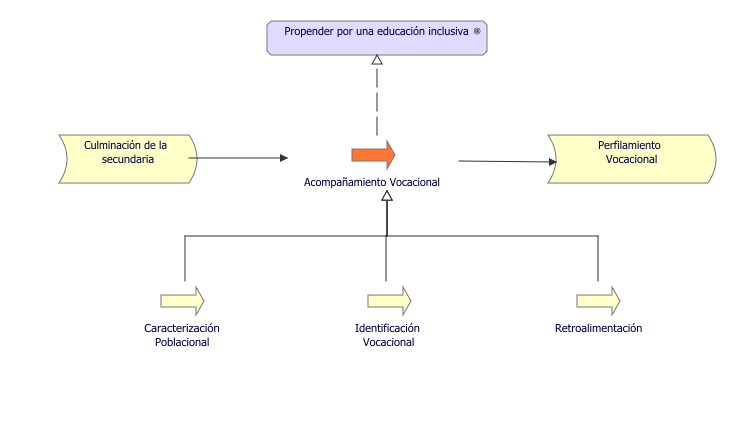
\includegraphics[width=.9\linewidth]{imgs/caso/negocio/ProcesoNegocio}
	\caption{Caso Proceso de Negocio}
\end{figure}

En el caso de nuestro proyecto, el proceso principal es el acompañamiento vocacional, vinculado al gran objetivo de propender por una educación inclusiva y dos eventos de negocio muy importantes que anteceden y preceden al proceso de negocio, el evento que antecede a este proceso de negocio es la culminación de la secundaria, posteriormente interviene el proceso de negocio con el acompañamiento vocacional y precede a este el evento de negocio del perfilamiento vocacional como finalización a este proceso, además este proceso principal está acompañado de tres subprocesos que en orden correspondiente son, en primer lugar la caracterización poblacional, continua con la identificación vocacional y finaliza con una retroalimentación.


\clearpage
\section{Punto de Vista de Cooperación de Proceso de Negocio}

El punto de vista de cooperación de proceso de negocio, promueve la identificación y asociación de roles a través de procesos, en otras palabras, es la vinculación existente entre los procesos y los roles, este punto de vista se deriva directamente del punto de vista de proceso de negocio y al identificar estos roles, permite expandir la forma en que se entiende el proyecto, asignando responsables a procesos.

\subsection{Modelo de Cooperación de Proceso de Negocio}
\begin{figure}[h!]
	\centering
	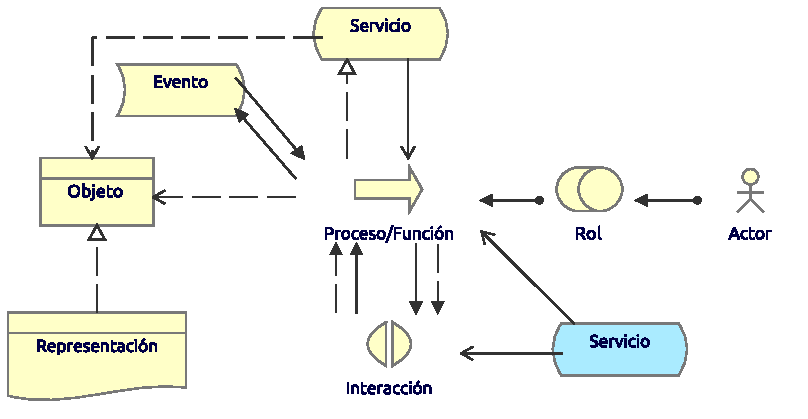
\includegraphics[width=.8\linewidth]{imgs/modelo/ProcesoNegocio}
	\caption{Modelo Cooperación de Proceso de Negocio}
\end{figure}

El modelo del punto de vista de Cooperación de Proceso de Negocio, se compone de un conjunto de partes, principalmente mencionadas en la parte exclusiva del proceso de negocio como lo son: el proceso o función, el evento, los derivados de este evento y proceso como el servicio, el objeto, la interacción y la representación y sin dejar de lado el enlace principal con el proceso el cual es el objetivo, estas partes componen tanto al punto de vista de proceso de negocio como al punto de vista de cooperación de proceso de negocio, a excepción que este segundo punto de vista incluye uno o varios roles, el cual se le asigna al proceso en cuestión.

\clearpage
\subsection{Caso de Cooperación de Proceso de Negocio}
\begin{figure}[h!]
	\centering
	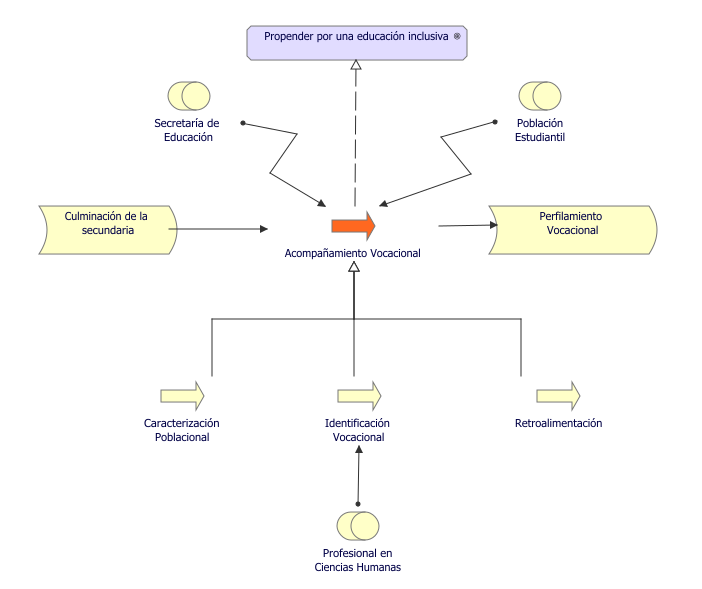
\includegraphics[width=.9\linewidth]{imgs/caso/negocio/CoopProNegocio}
	\caption{Caso Cooperación de Proceso de Negocio}
\end{figure}

Este proyecto de colaboración con el Ministerio de Educación Nacional para tener una educación inclusiva y contribuir con el mejoramiento de la educación en el territorio nacional, posee un gran objetivo el cual es el propender por una educación inclusiva, del cual se deriva el proceso principal de tener un acompañamiento vocacional que lo antecede el evento de negocio de la culminación de la secundaria y lo precede el evento del perfilamiento vocacional, a este gran proceso se le asignan dos roles que intervienen en el, como lo son: la secretaría de educación y la población estudiantil además, este proceso principal cuenta con tres sub procesos: la caracterización poblacional, la identificación vocacional que está vinculada con el rol de los profesionales en ciencias humanas y el subproceso de la retroalimentación.


\clearpage
\section{Punto de Vista de Producto}


\subsection{Modelo de Producto}
\begin{figure}[h!]
	\centering
	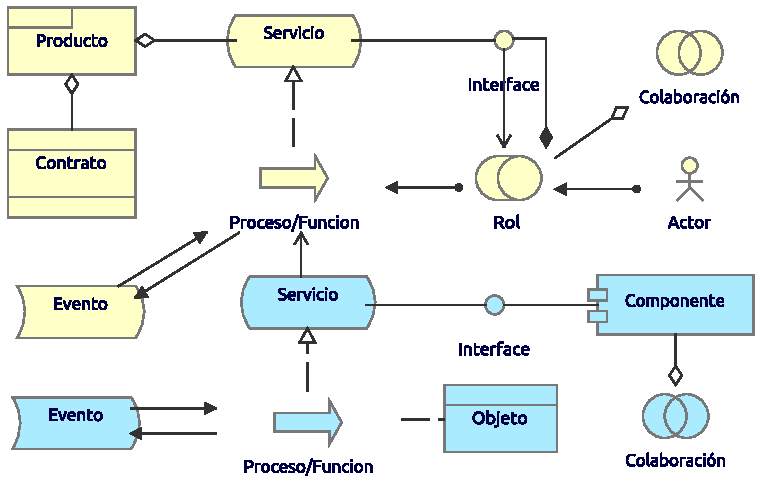
\includegraphics[width=.6\linewidth]{imgs/modelo/Producto.pdf}
	\caption{Modelo Producto}
\end{figure}

El punto de vista de producto permite ver el conjunto de contratos que rigen un producto de la organización, además relaciona los servicios que se desprenden del producto. Estos contratos son aquello que regulan y limitan  al producto. Los servicios asociados al producto son parte de los objetivos, misión y visión de la empresa y que desembocan en proceso de la organización ya sea implícito o explícito relacionado obviamente con el producto.

\newpage
\subsection{Caso  de Producto}
\begin{figure}[h!]
	\centering
	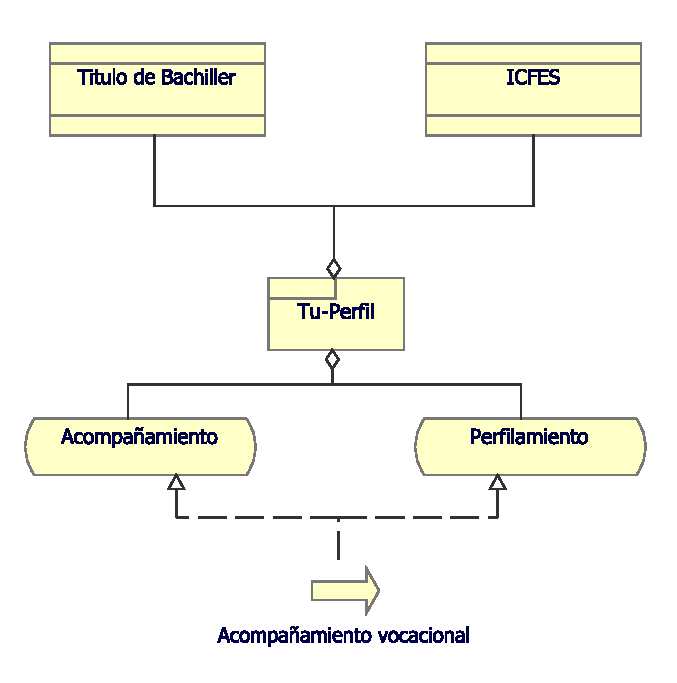
\includegraphics[width=.9\linewidth]{imgs/caso/negocio/producto.pdf}
	\caption{Caso Producto}
\end{figure}

Para el caso de estudio tenemos como producto de negocio a Tu-Perfil aquel apartado que servirá como guiá para acompañar y perfilar a los estudiantes en la elección de vocación que sera tomada al graduarse como bachiller con el fin de dar cabida al proceso de acompañamiento vocacional que surge de los objetivos de la organización para este caso el MEN.  Este producto esta regido por los contratos definidos ICFES y Titulo de Bachiller, que serán aquellos que limitaran al producto.
